\chapter{Use Cases}
\label{cap:UseCases} 


\section{Initialization}
The first time the appliction is opened the user sees a welcome message and his
prompted to comlete the initialization wizard which consists in selecting and
confirming a password which will be the one needed by other telephones/users
to send commands to that mobile. The password scheme forces to select an
alphanumeric string (some special characters are also allowed) between 8-
20 characters and with at least a letter and a number. In case of error
(bad password/confirmation password different from the base one) the user is
notified back and asked to retry. In case of success the application redirects
to the main view, which is the "sms localization" one.

\subsection{Activity Diagram}

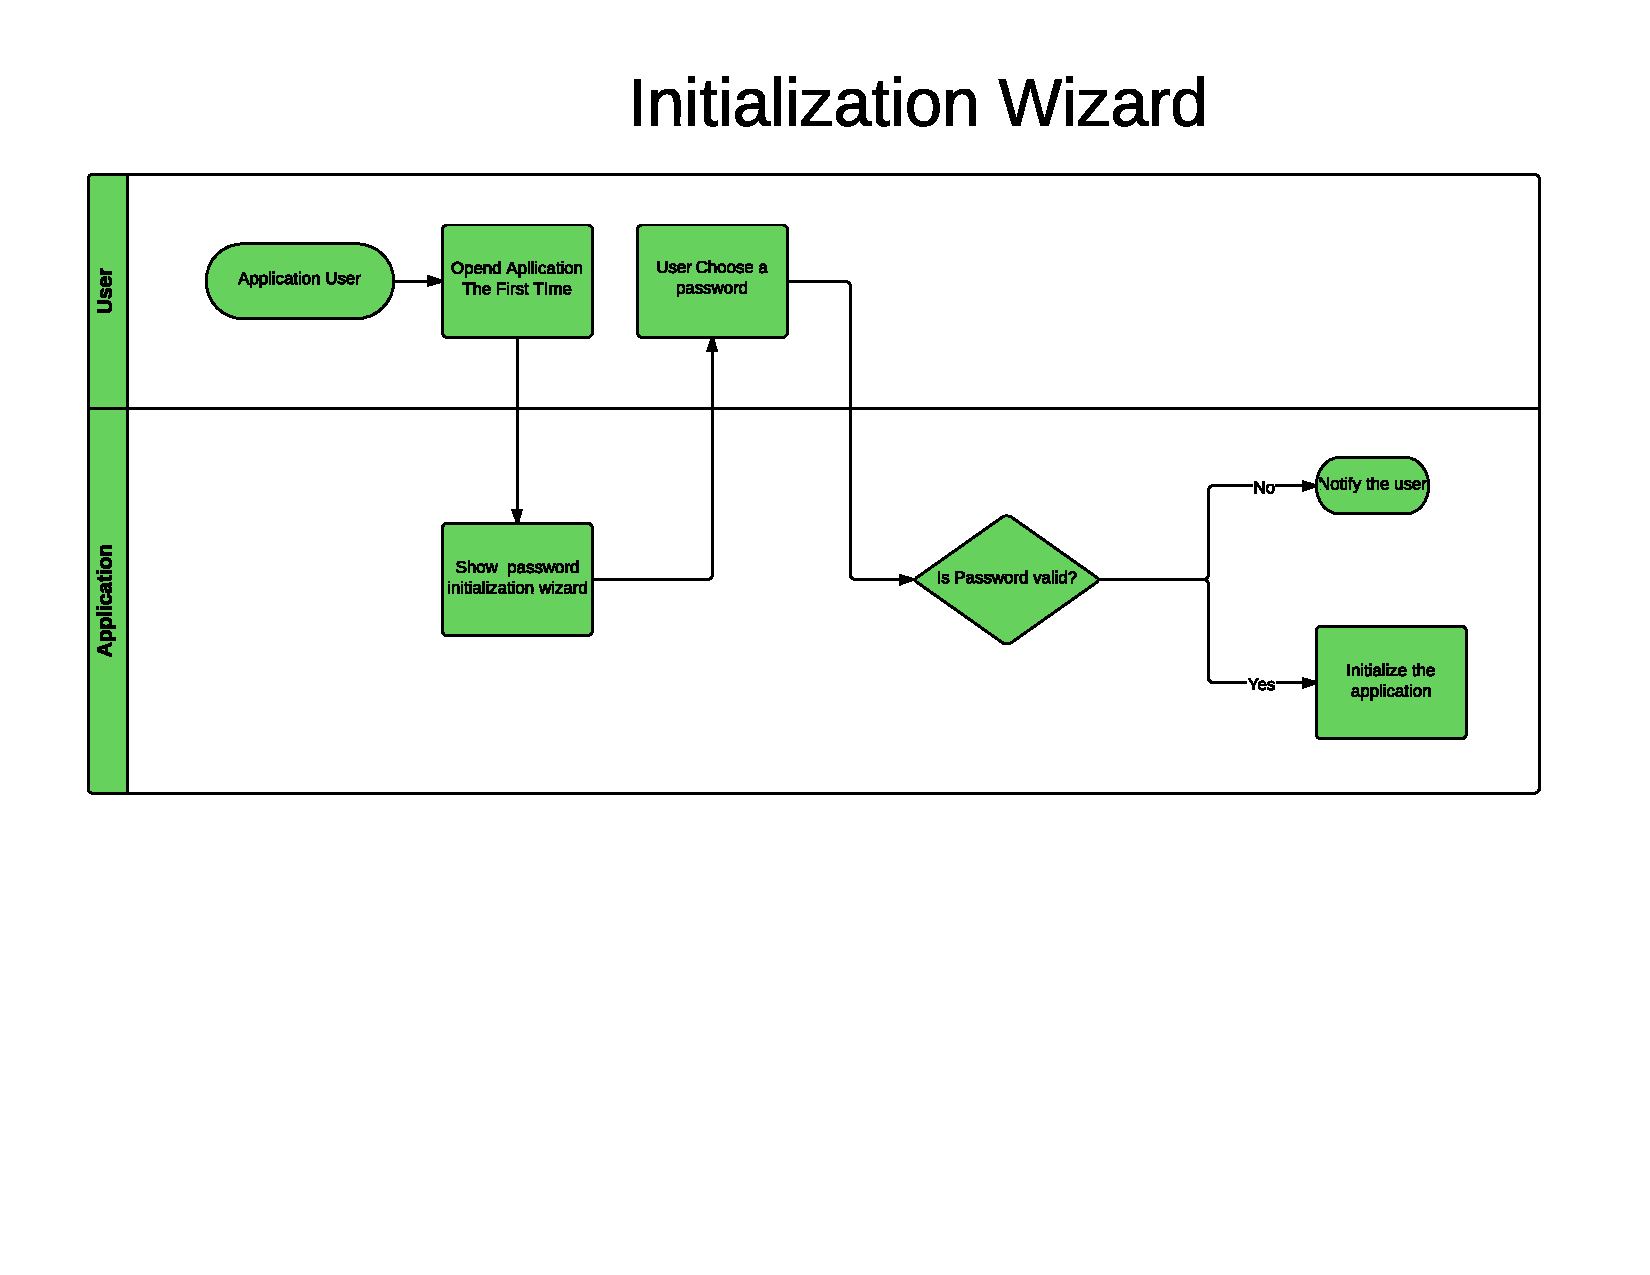
\includegraphics[scale=0.5]{images/initialization_activity}

\newpage
\subsection{User Interface Design}

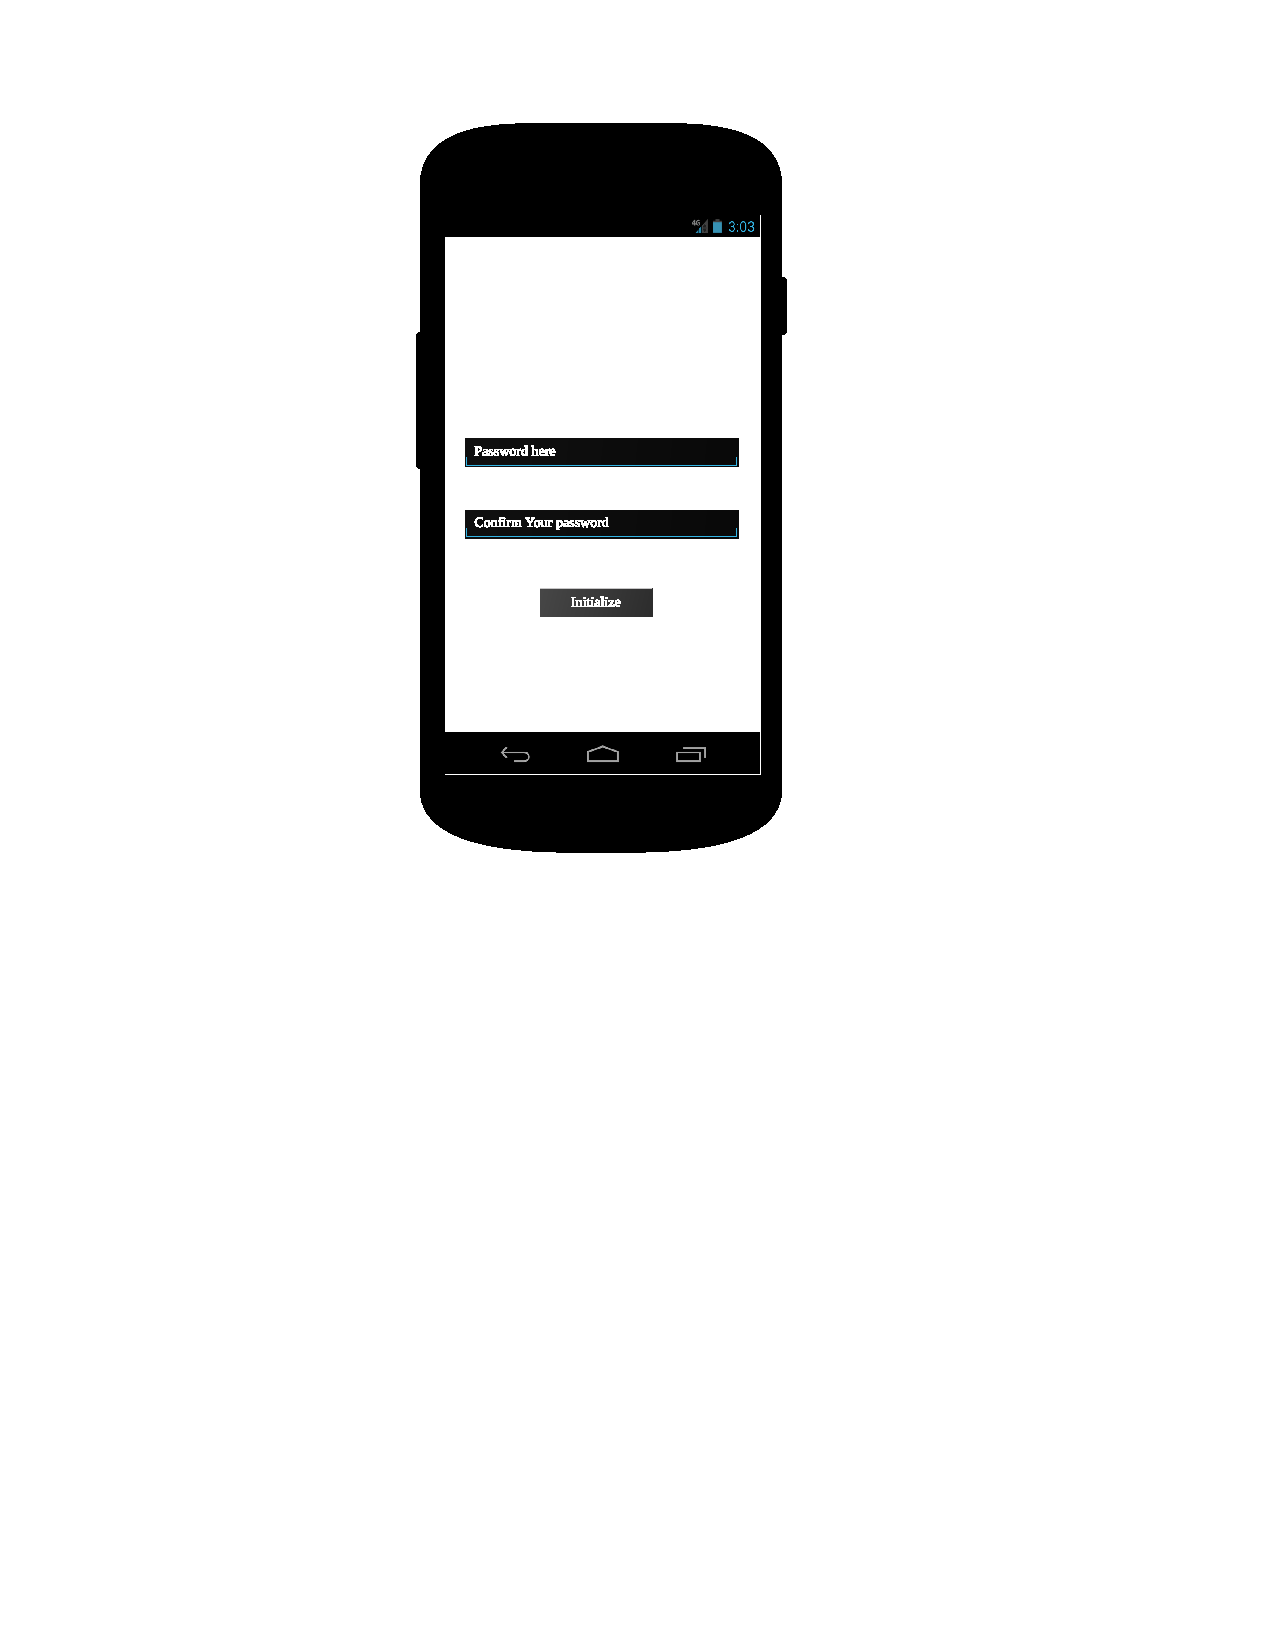
\includegraphics[scale=0.7]{images/initialization_design}


\section{Mobile Phone Association}
For enhanced security it’s required two telephones are associated before they
can send commands to the other one; the association is bidirectional and can
be removed only locally (the other telephone won’t know anything, but will
obviously fail in sending commands). This totally cuts away the possibility of
a Man In The Middle (MITM) both active and passive. A user who wants
to associate his telephone with another one first selects a secret question
and a secret answer and sends the first to the other mobile, whose user can
decide to accept or refuse the request. In the second case the first user is
notified back and the association ends with a "failure", otherwise the second
user types what he thinks is the secret answer and selects his own secret
question/answer. The first user now has to type the answer to that question
and, if all goes smooth, the association is done. Every passage is done by
sms sending.

\newpage
\subsection{Activity Diagram}

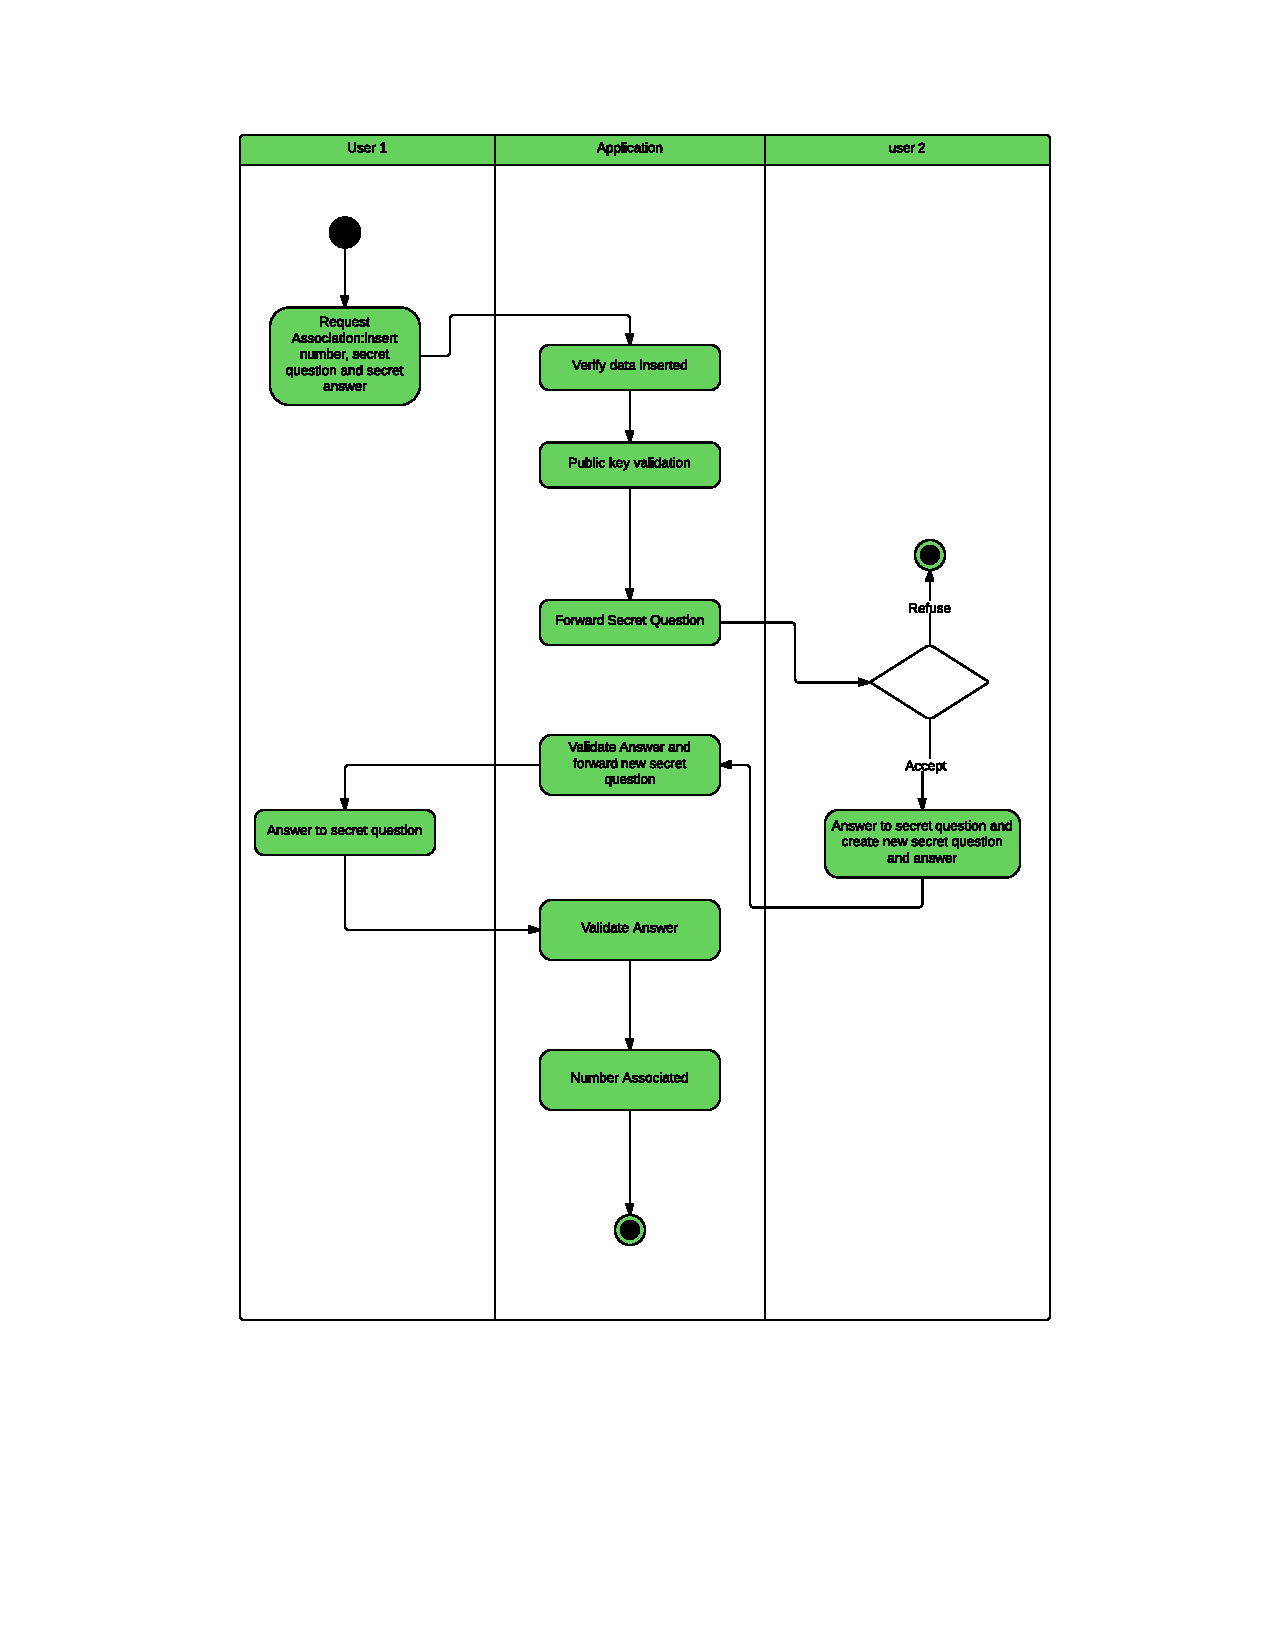
\includegraphics[scale=0.7]{images/SMP_activity}

\newpage
\subsection{User Interface Design}

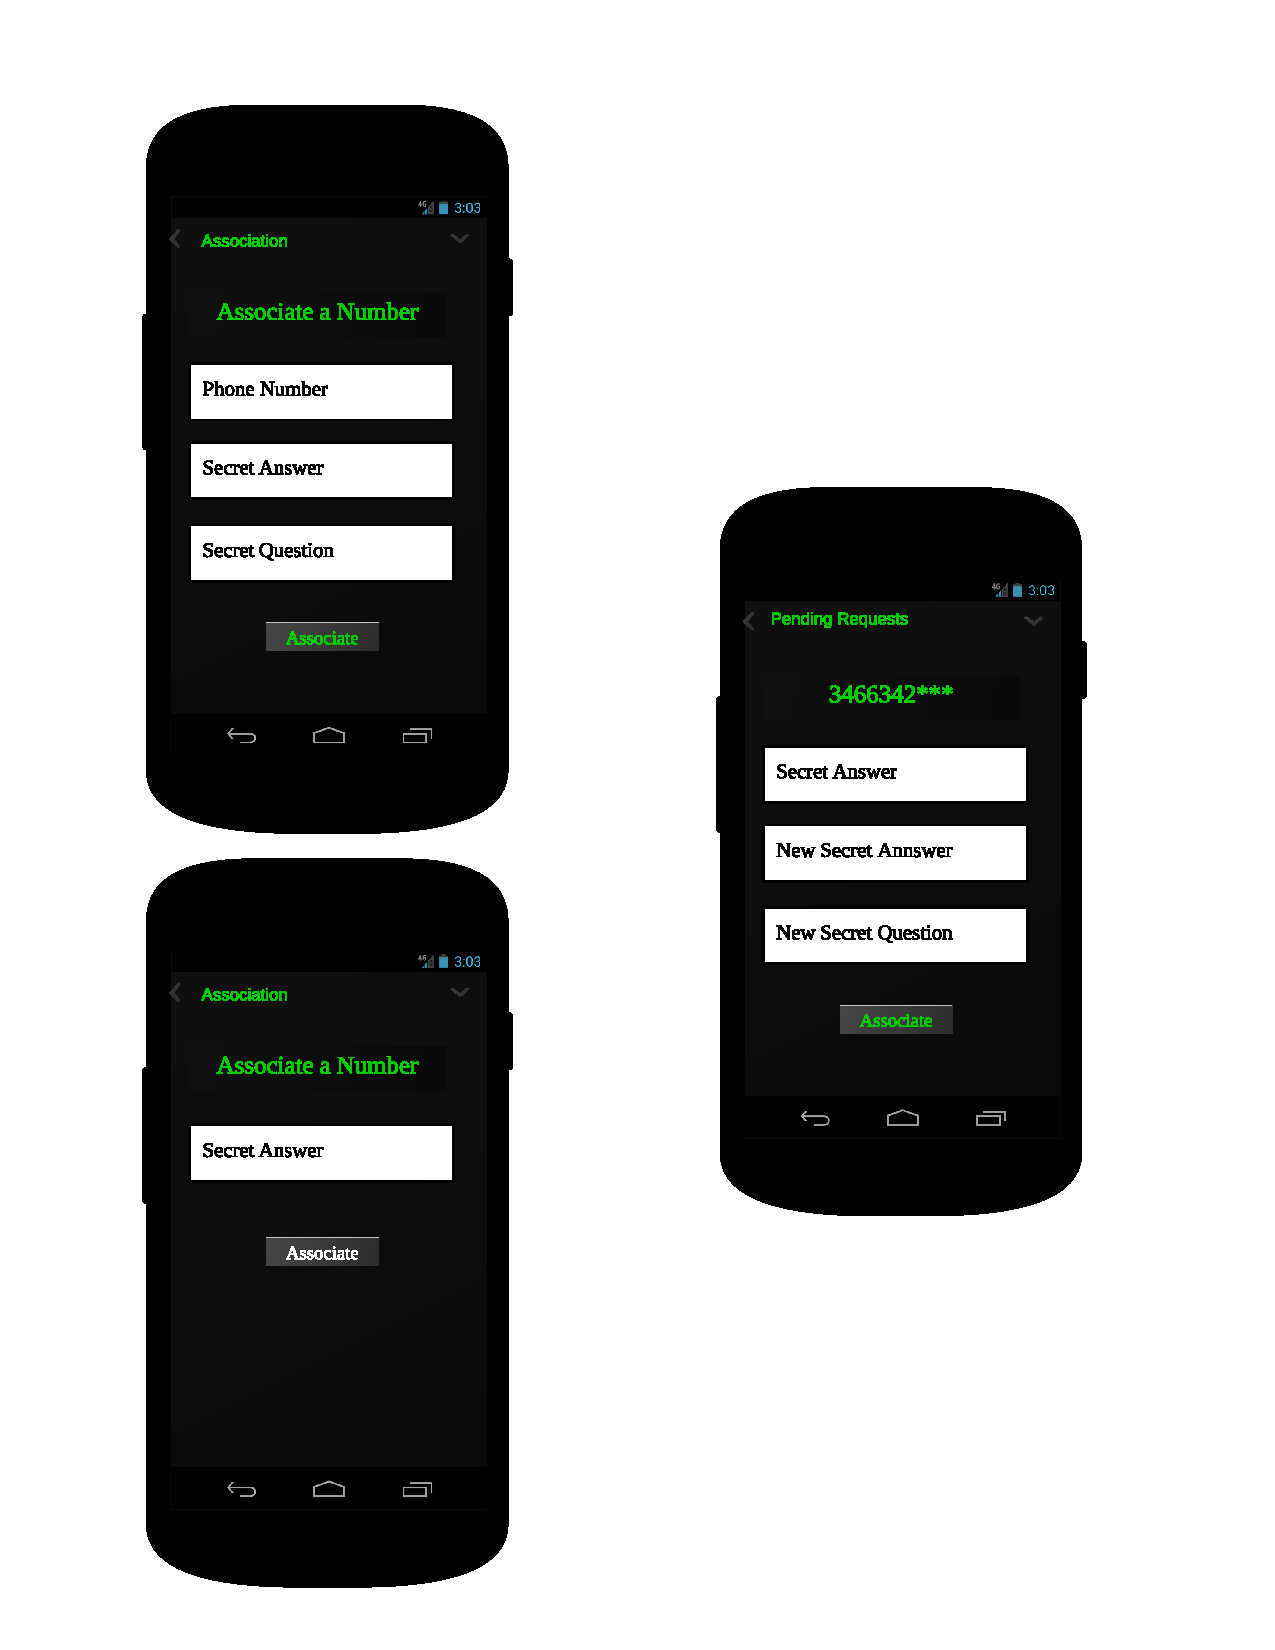
\includegraphics[scale=0.7]{images/SMP_design}

\section{Password Change}

The user types the old password, the new password and the confirmation new
password; the system checks whether the old one is correct and the new ones
are coherent and rules compliant (see initialization wizard use case). If not
an error message is prompted and nothing is done, otherwise the password is
succesfully updated and the user notified back.

\subsection{Activity Diagram}

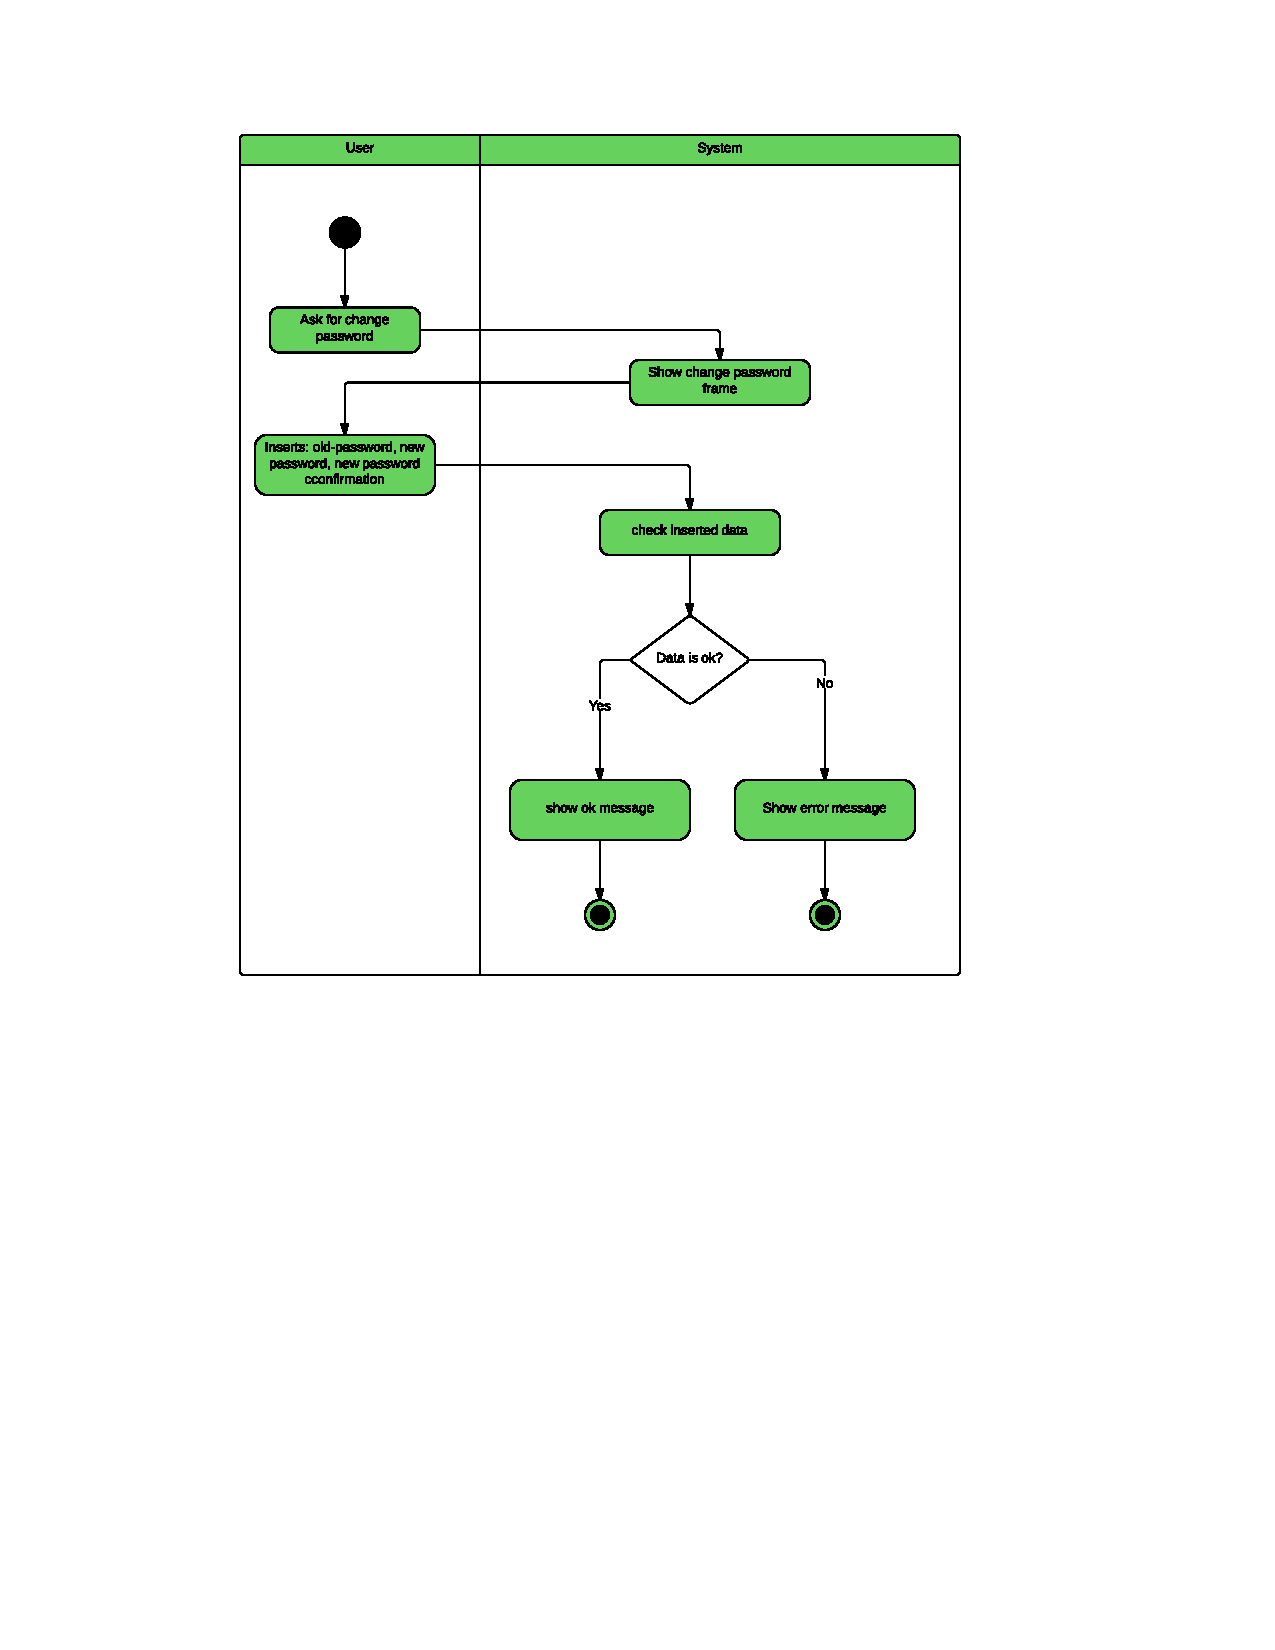
\includegraphics[scale=0.6]{images/ChangePassword_activity}

\newpage
\subsection{User Interface Design}

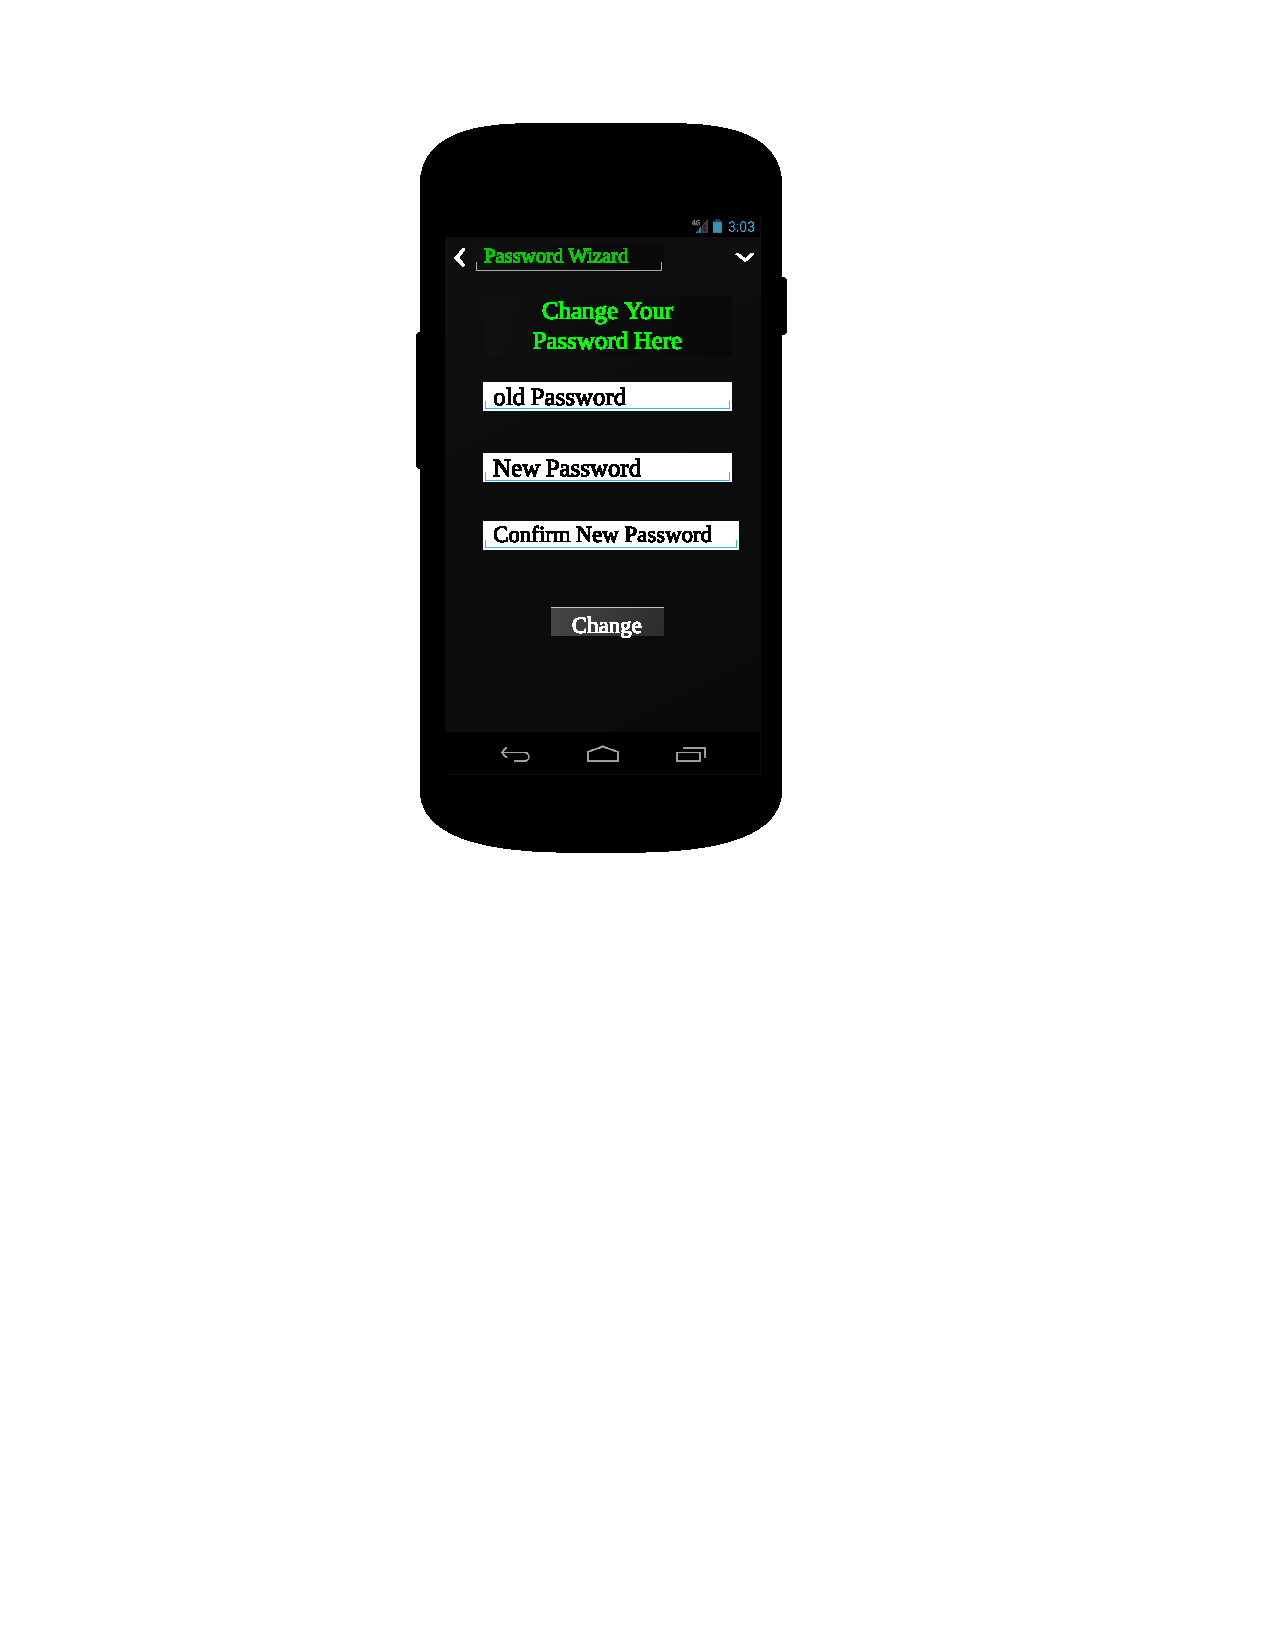
\includegraphics[scale=0.7]{images/PasswordChange_UI}

\section{Unilateral Deassociation}

The user selects from the list of his contacts the one he wants to deassociate
with and confirms his intention by clicking on the apposite button. The
relative preferences are deleted, but the "target" is not notified.


\newpage
\subsection{Activity Diagram}

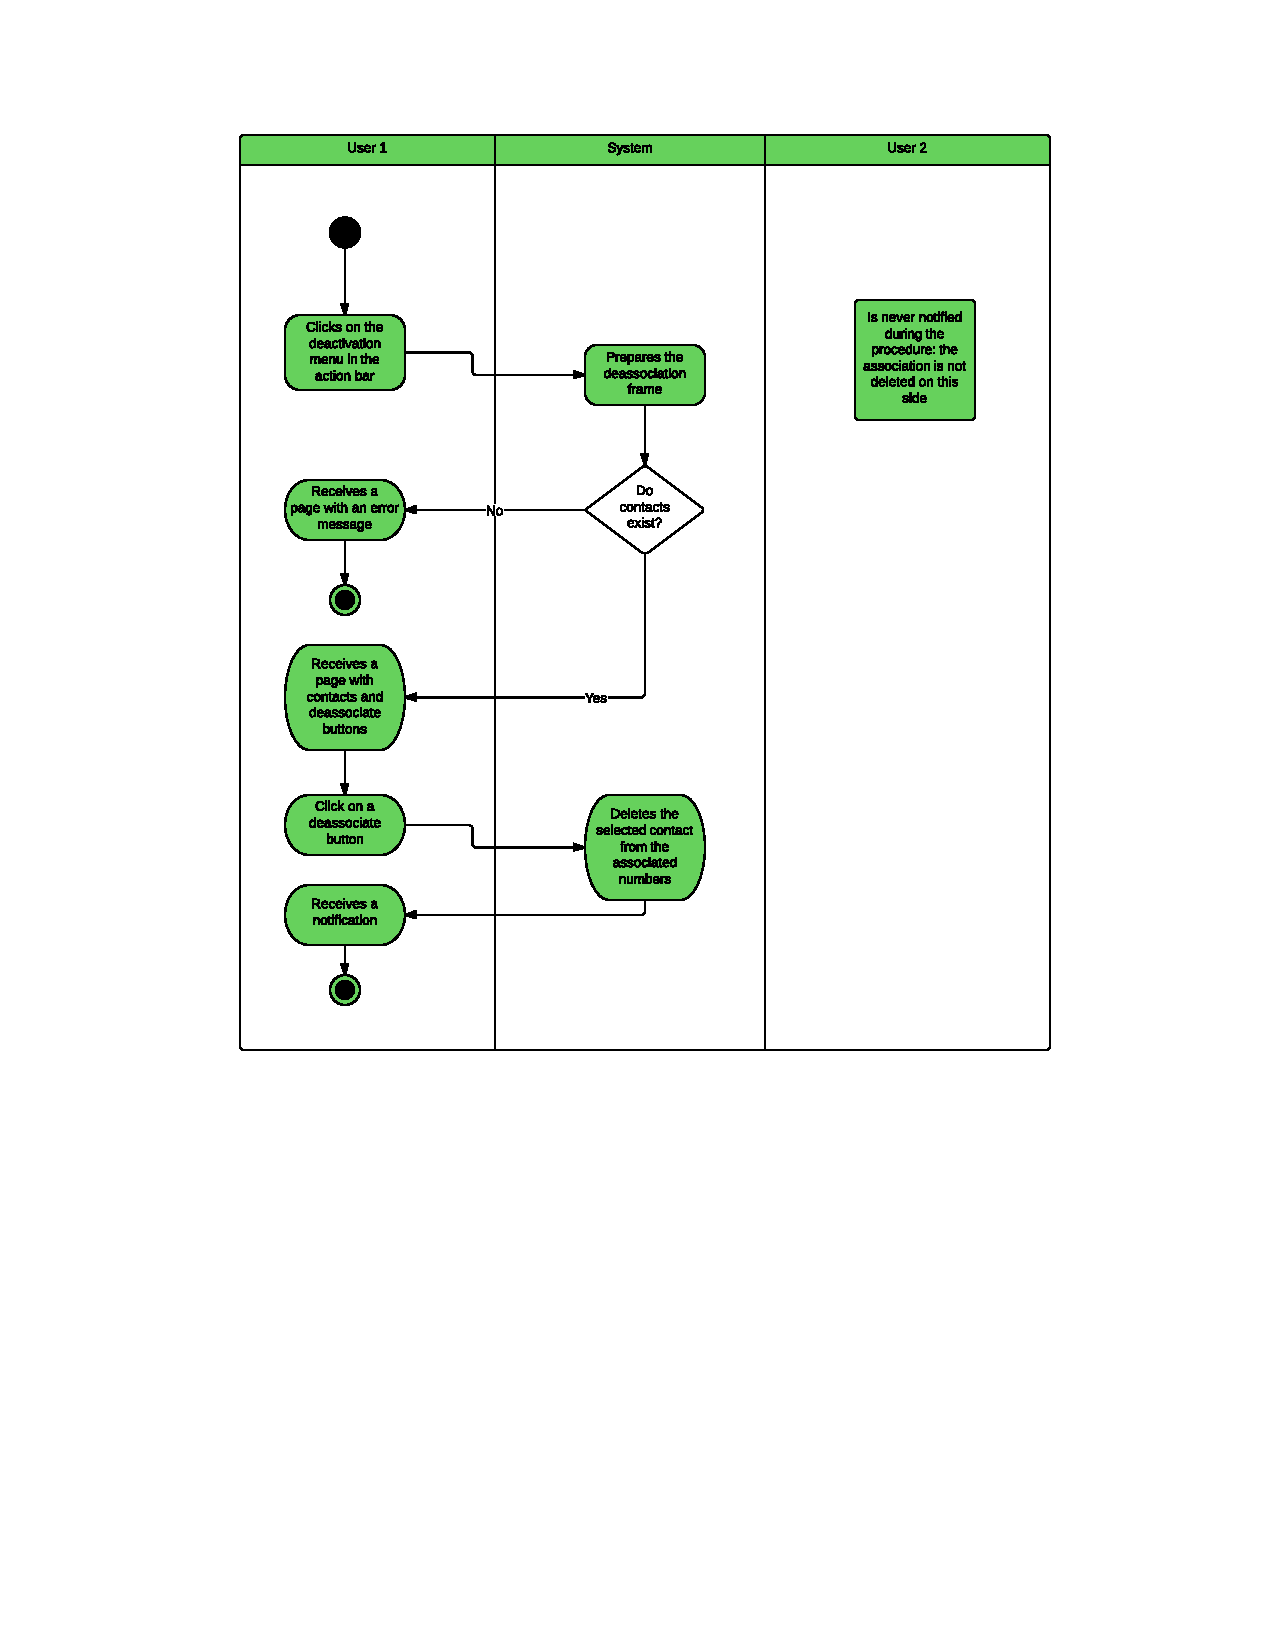
\includegraphics[scale=0.7]{images/UnilateralDeassociation}

\newpage
\subsection{User Interface Design}

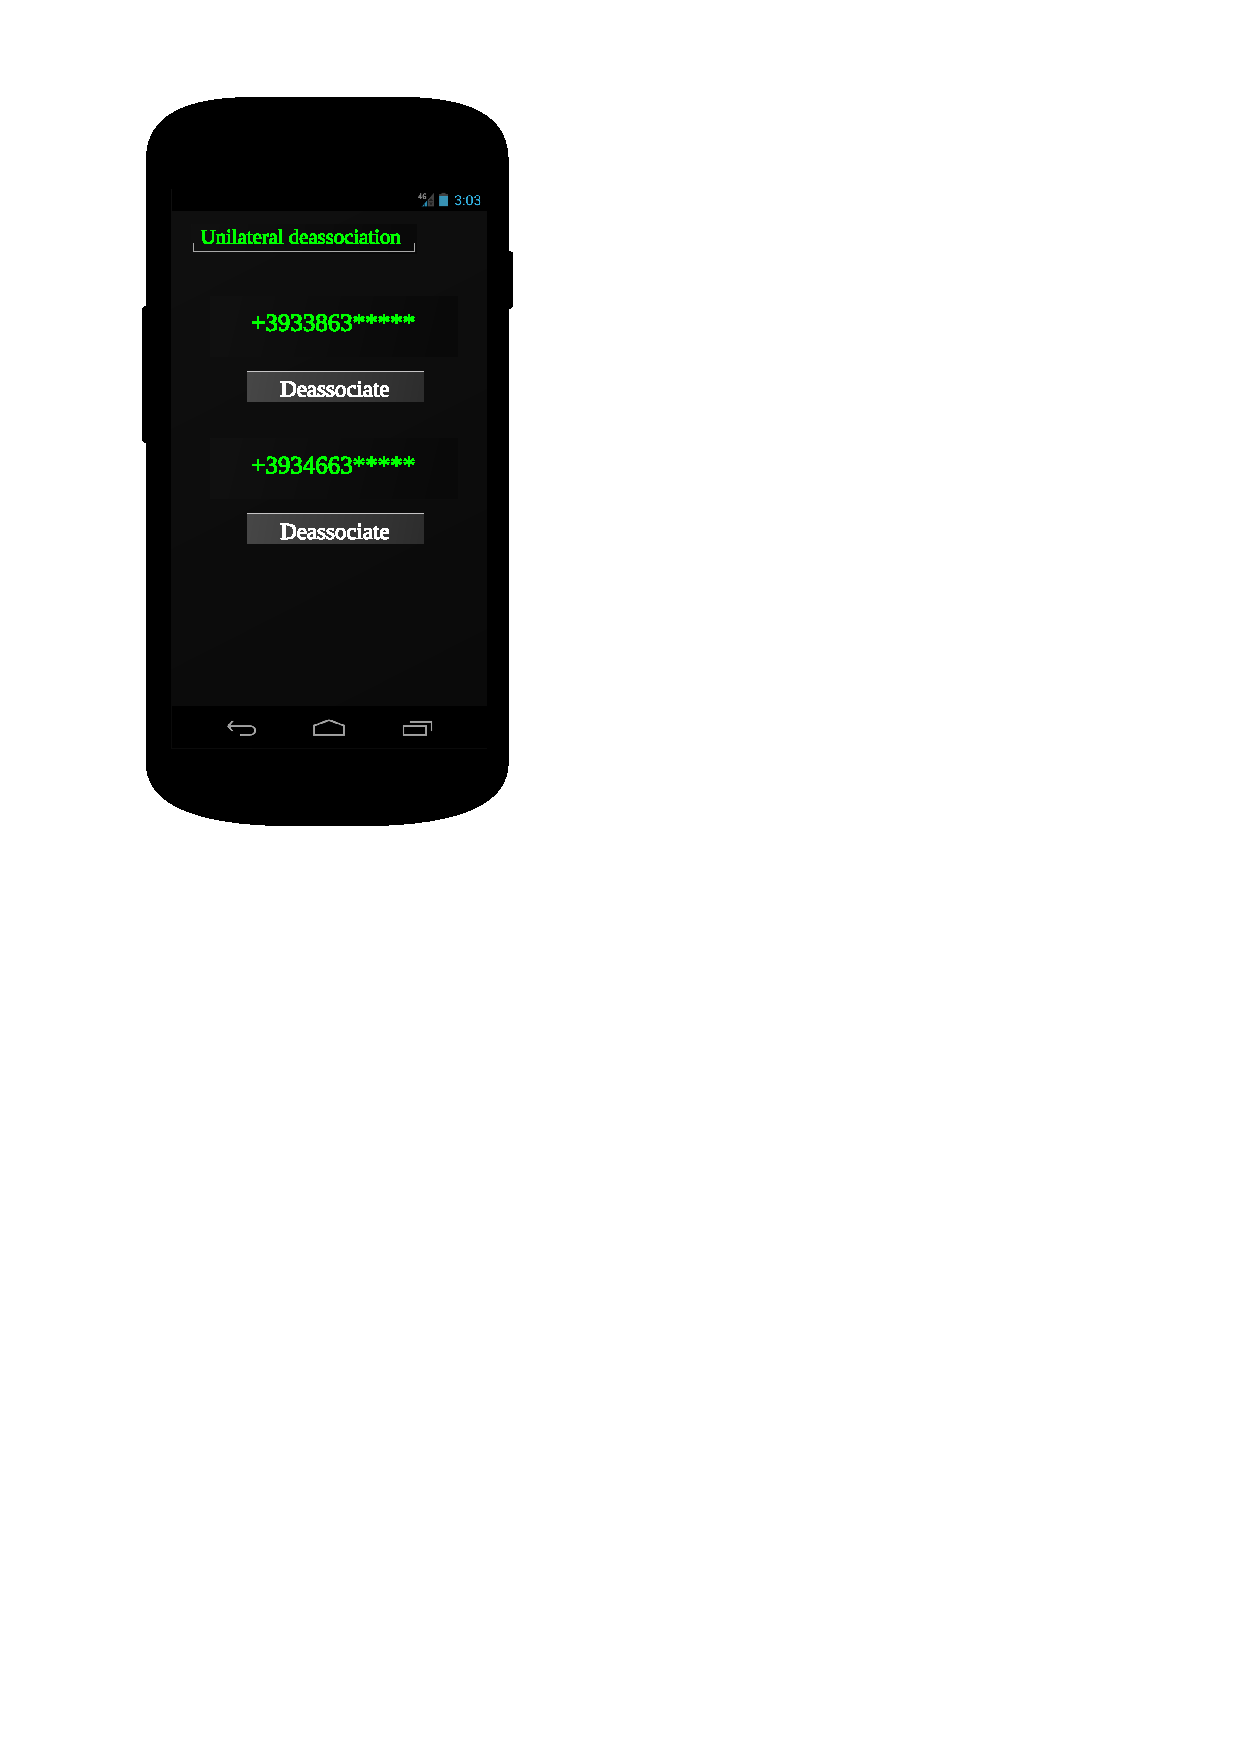
\includegraphics[scale=0.7]{images/DeassociationAndroid}

\section{Remote Localization}

The user (which sees a list of his contacts/associated numbers) types the
target password and confirms the intention to send a localize command by
clicking on the apposite button. After an handshake (done by sms exchanging)
the target phone executes the command and sends back a failure message or
his actual coordinates. The original sender receives a notification with a map
and a marker indicating the target position.


\newpage
\subsection{Activity Diagram}

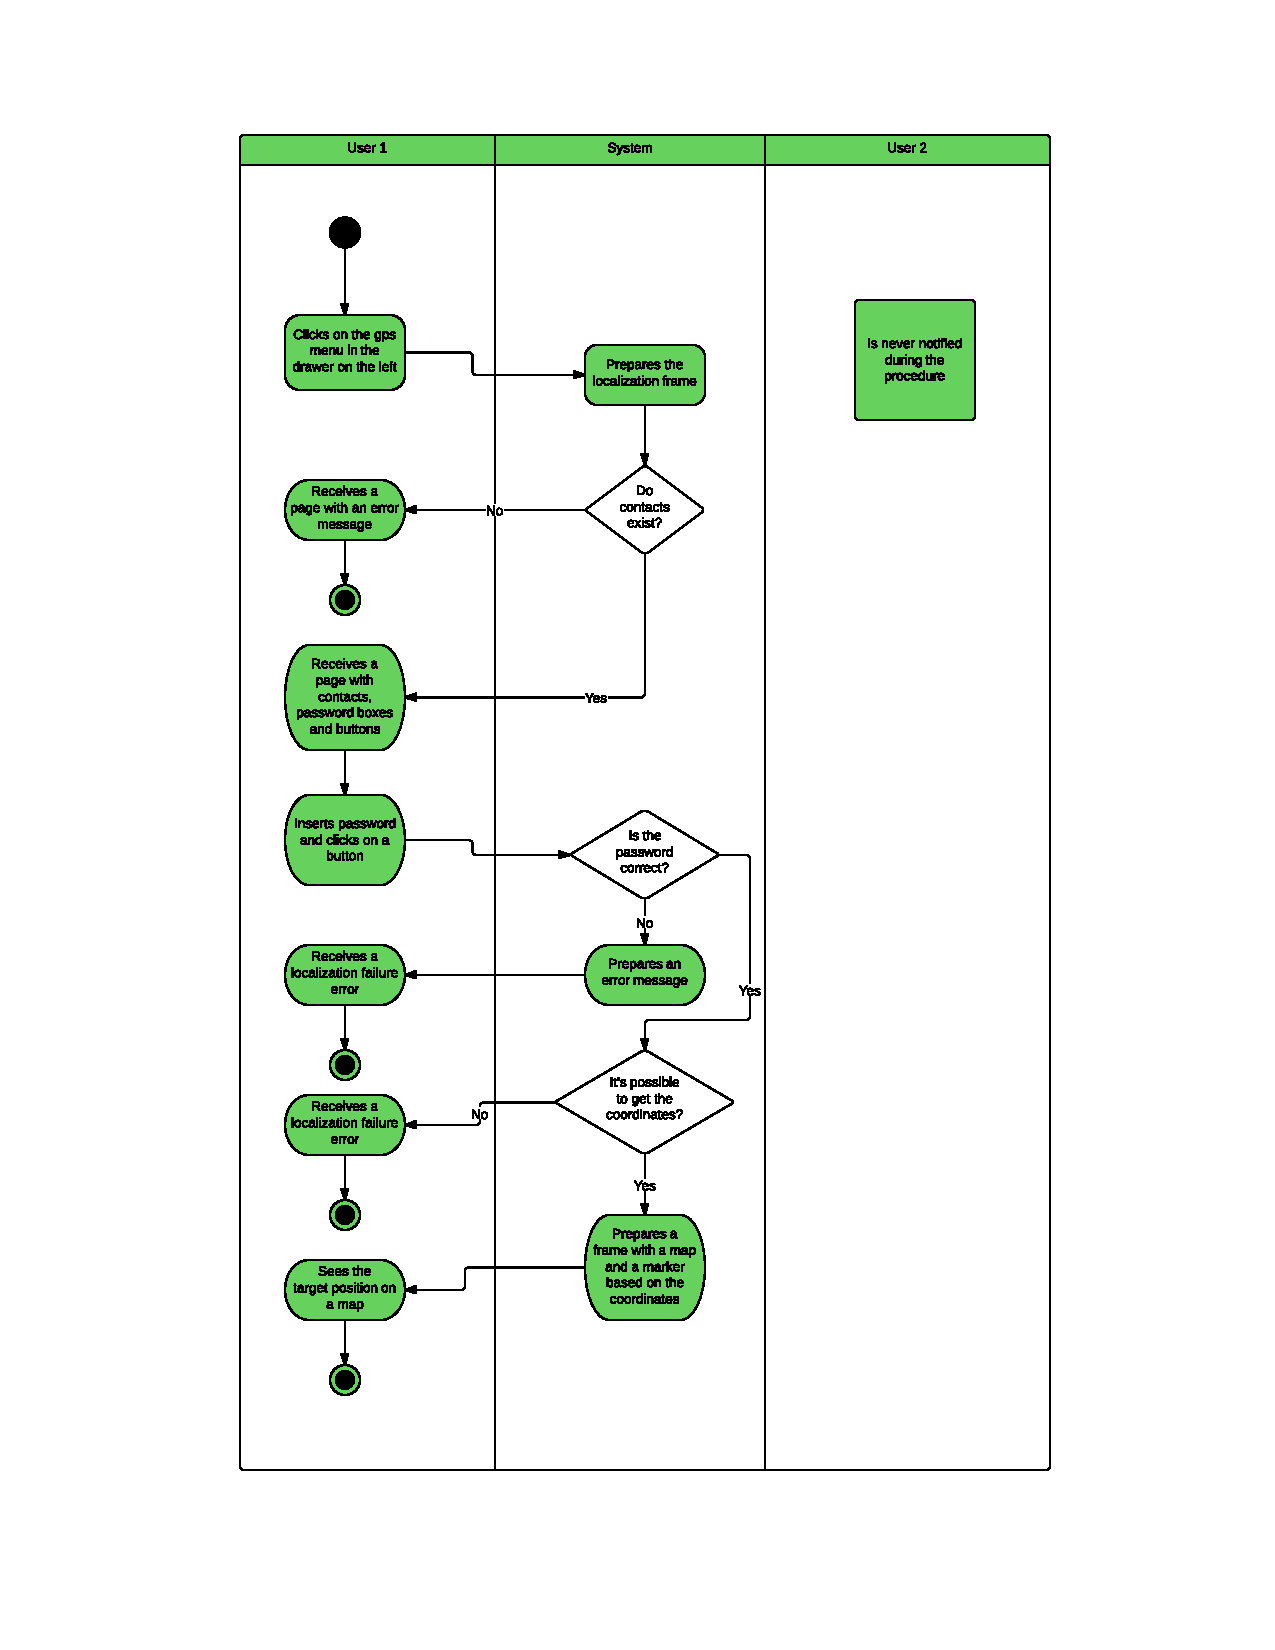
\includegraphics[scale=0.7]{images/Localization}

\newpage
\subsection{User Interface Design}

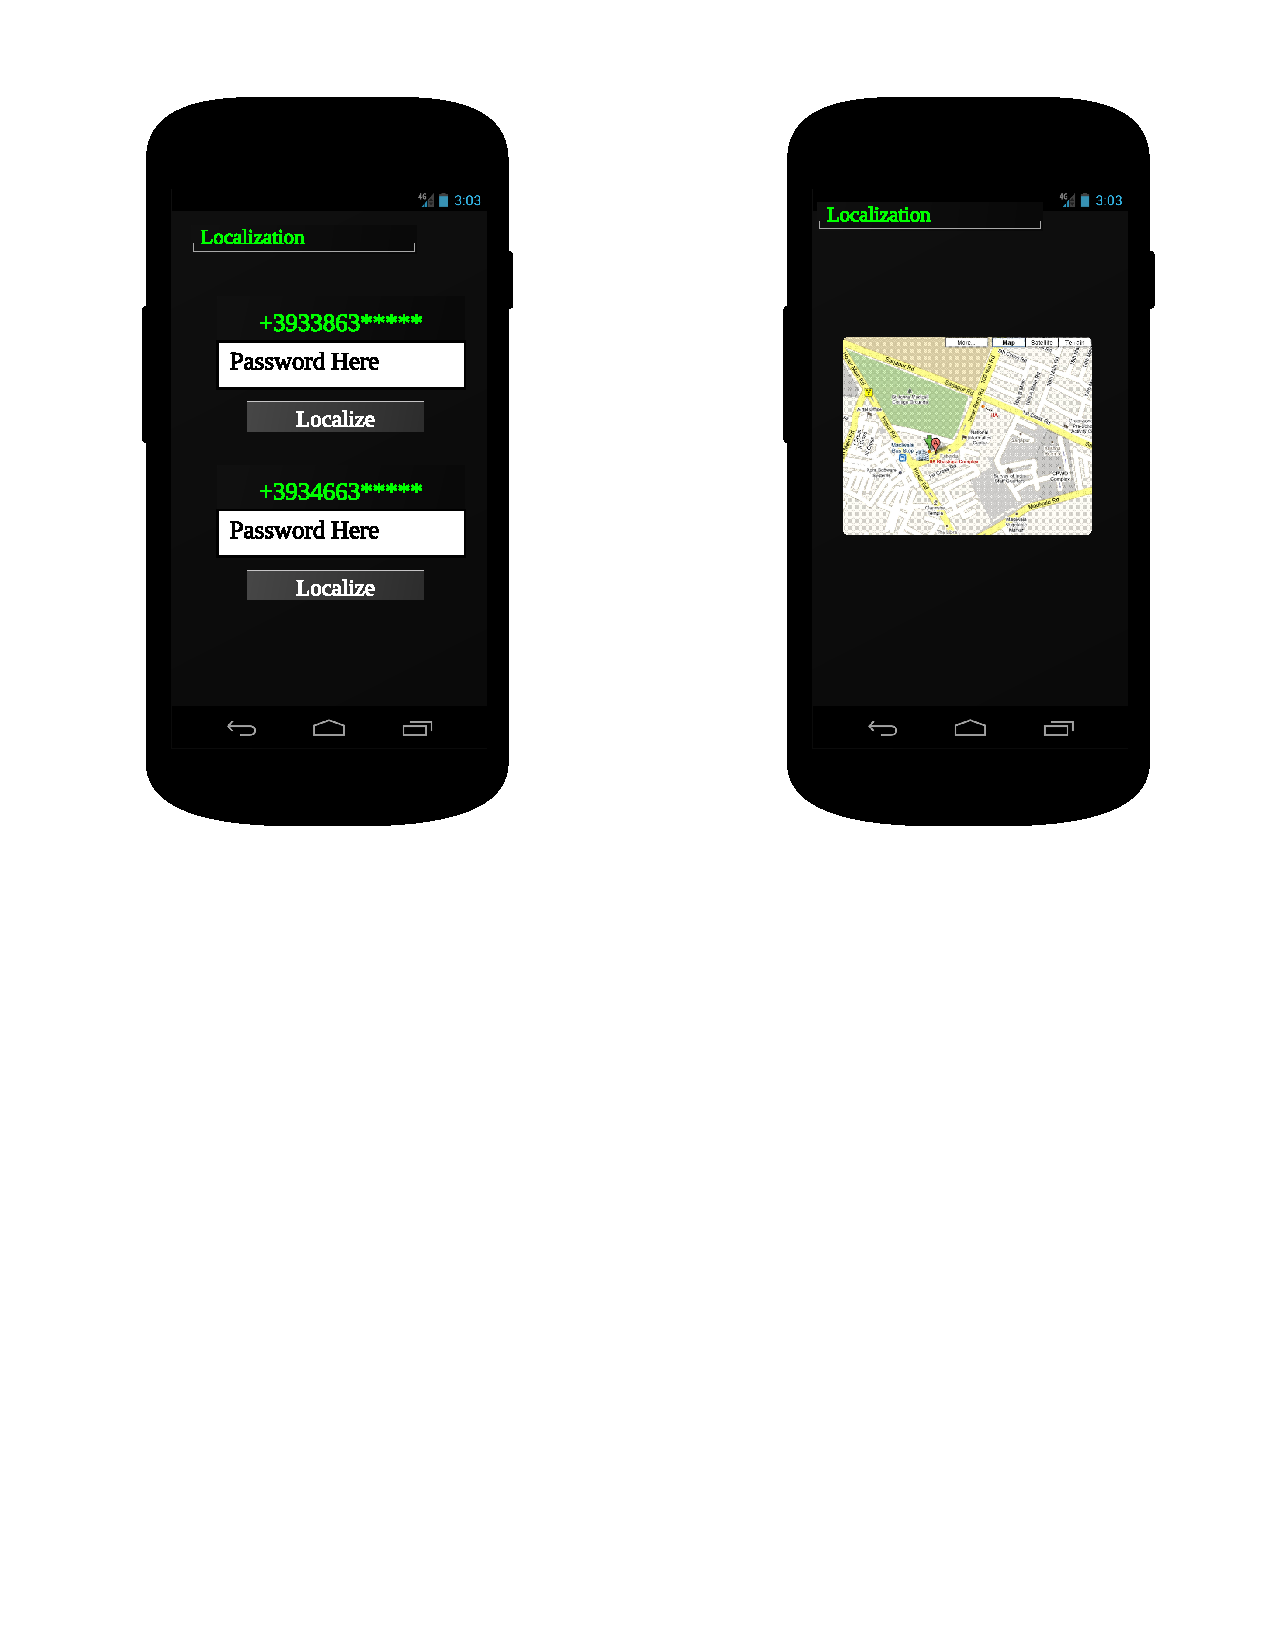
\includegraphics[scale=0.7]{images/Localization_mobile}

\section{Mobile Phone Mark}
The mark features have been left unimplemented: they are in the TODO list,
so no use cases for now.


\newpage
%\subsection{Activity Diagram}

%\newpage
%\subsection{User Interface Design}

\section{Remote Alarm Triggering: Activate and Deactivate Siren}

The user selects from his contacts the target and confirms by clicking on a
specific button the will to send a siren on/siren off command. The command
session is similar to the localization one: the only difference is that the re-
turned message is only an ack or a failure code. The siren off is simply ignored
if the alarm in not active. There is also a feature which allows a user to turn
off locally a siren by inserting the password and clicking on the button.

\newpage
\subsection{Activity Diagram}

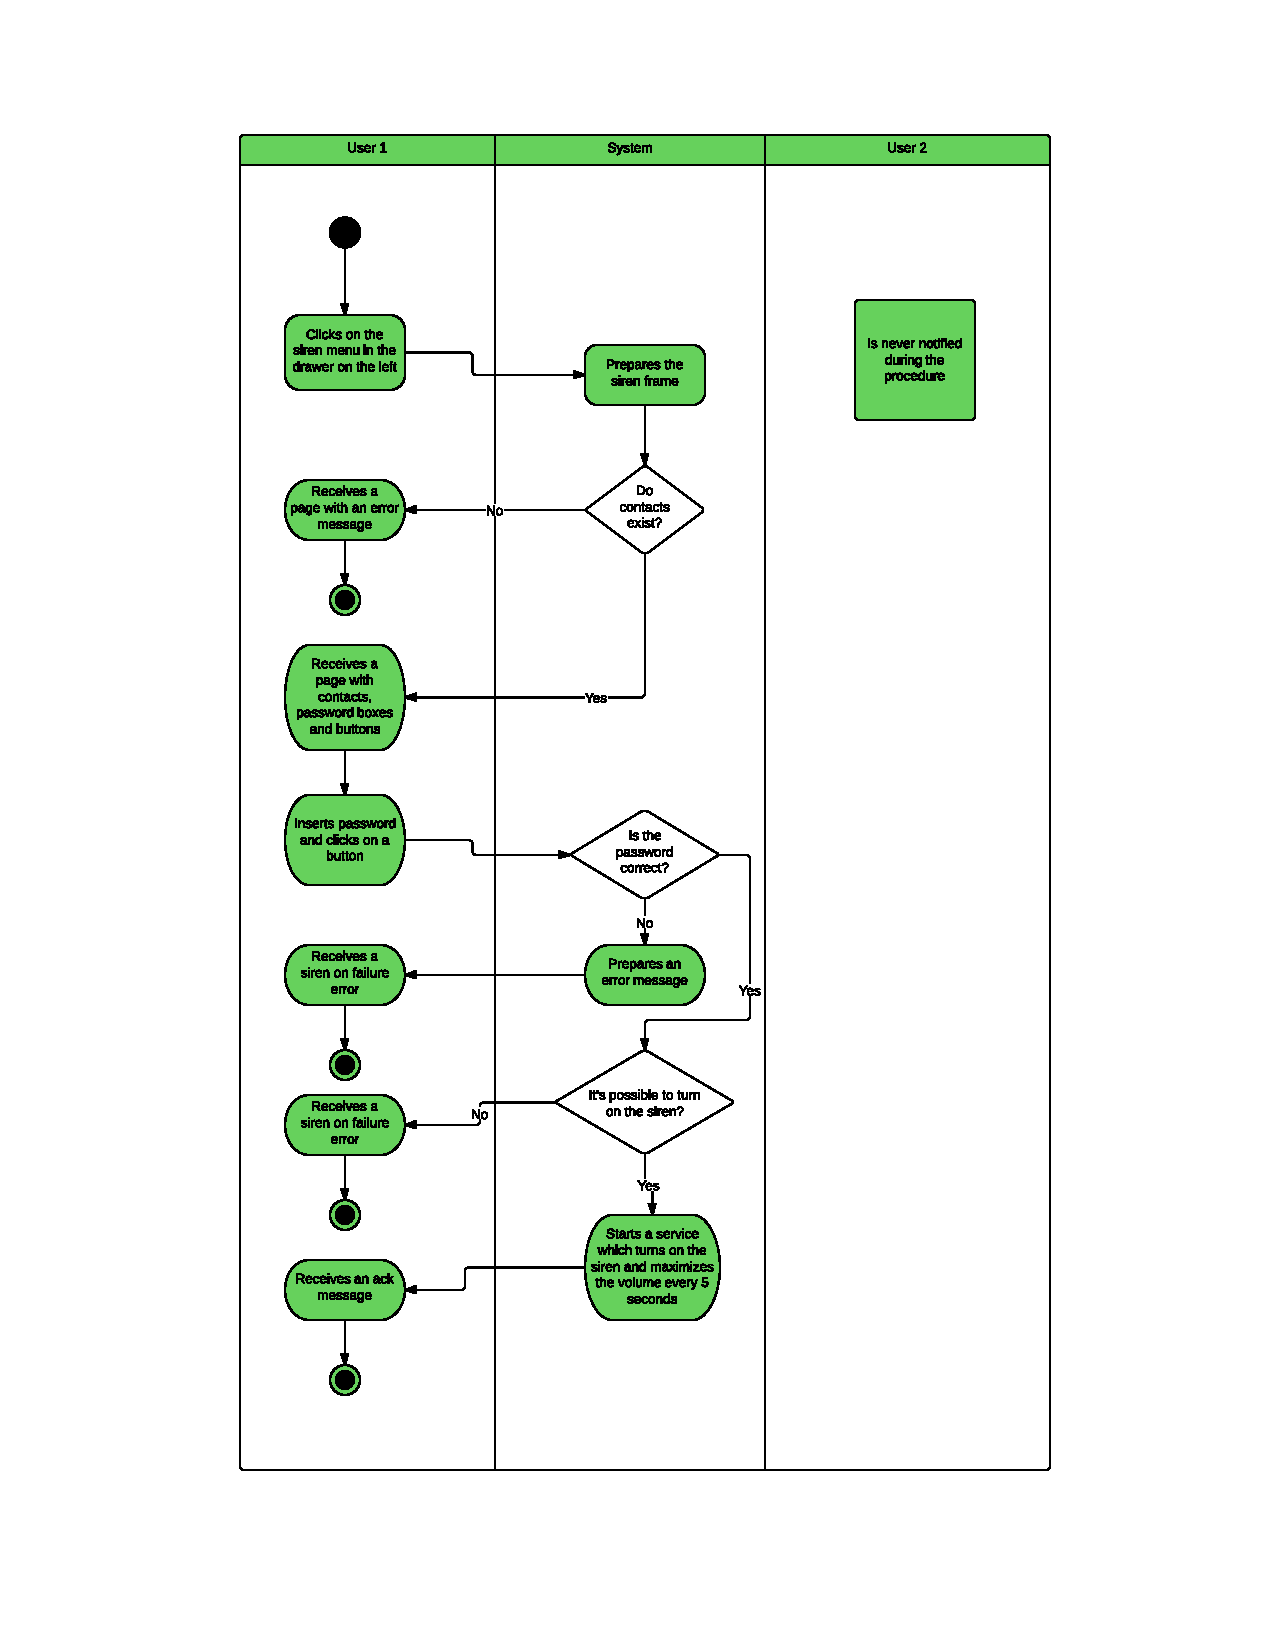
\includegraphics[scale=0.7]{images/SirenOn}
\newpage
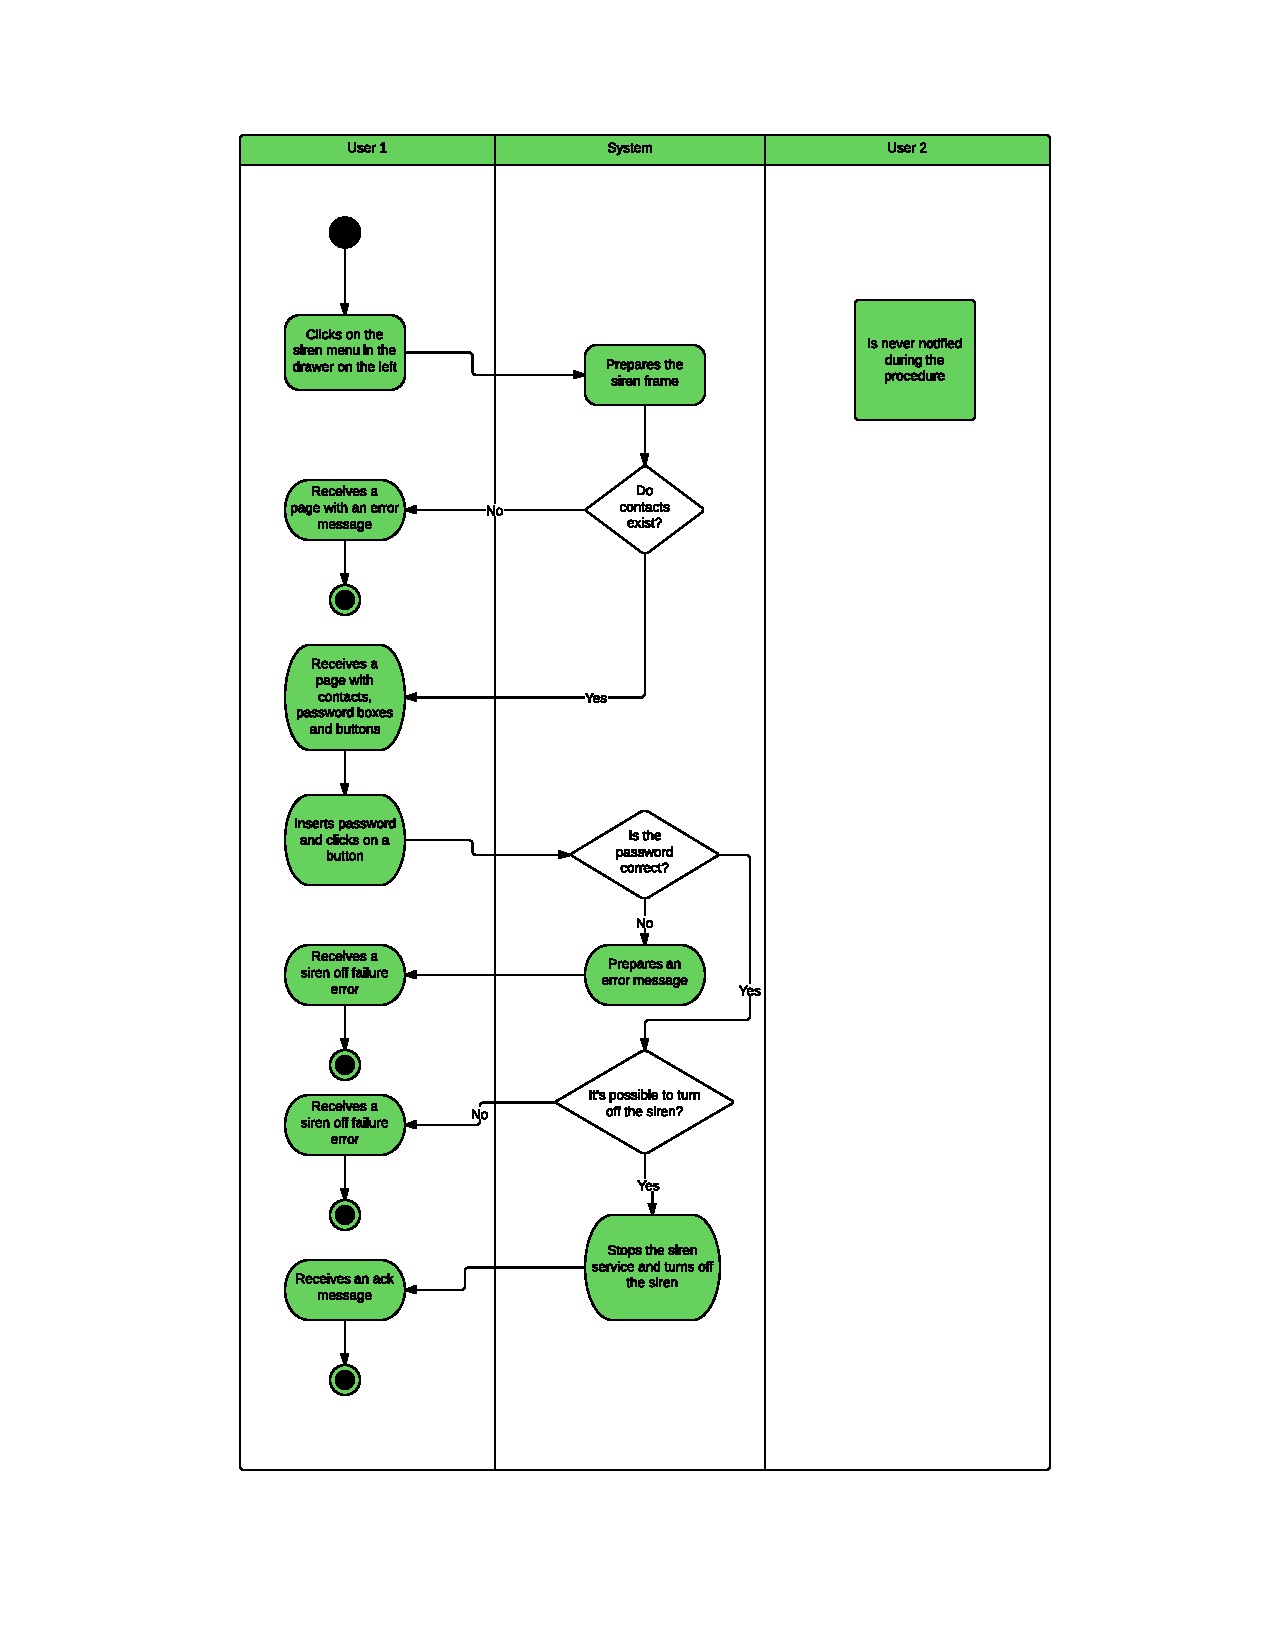
\includegraphics[scale=0.7]{images/SirenOff}
\newpage
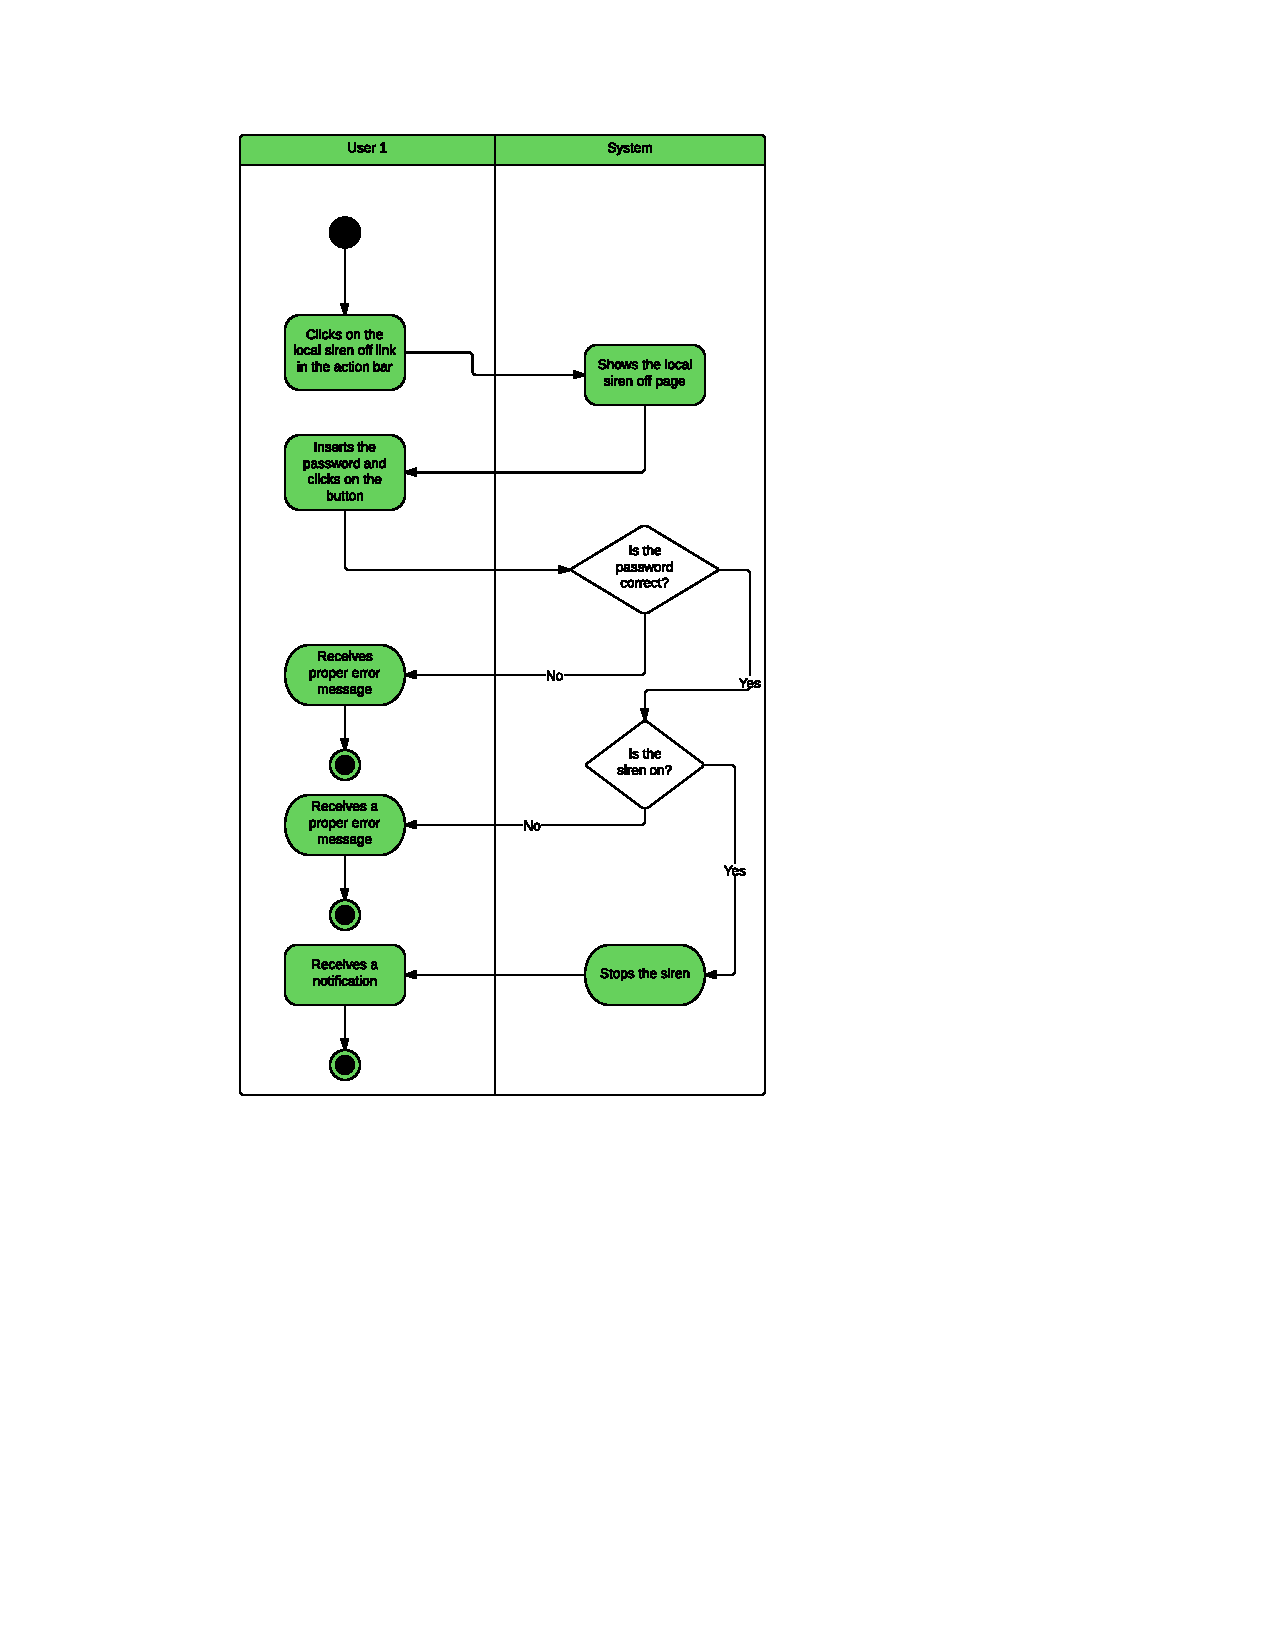
\includegraphics[scale=0.7]{images/localsirenoff}

\newpage
\subsection{User Interface Design}

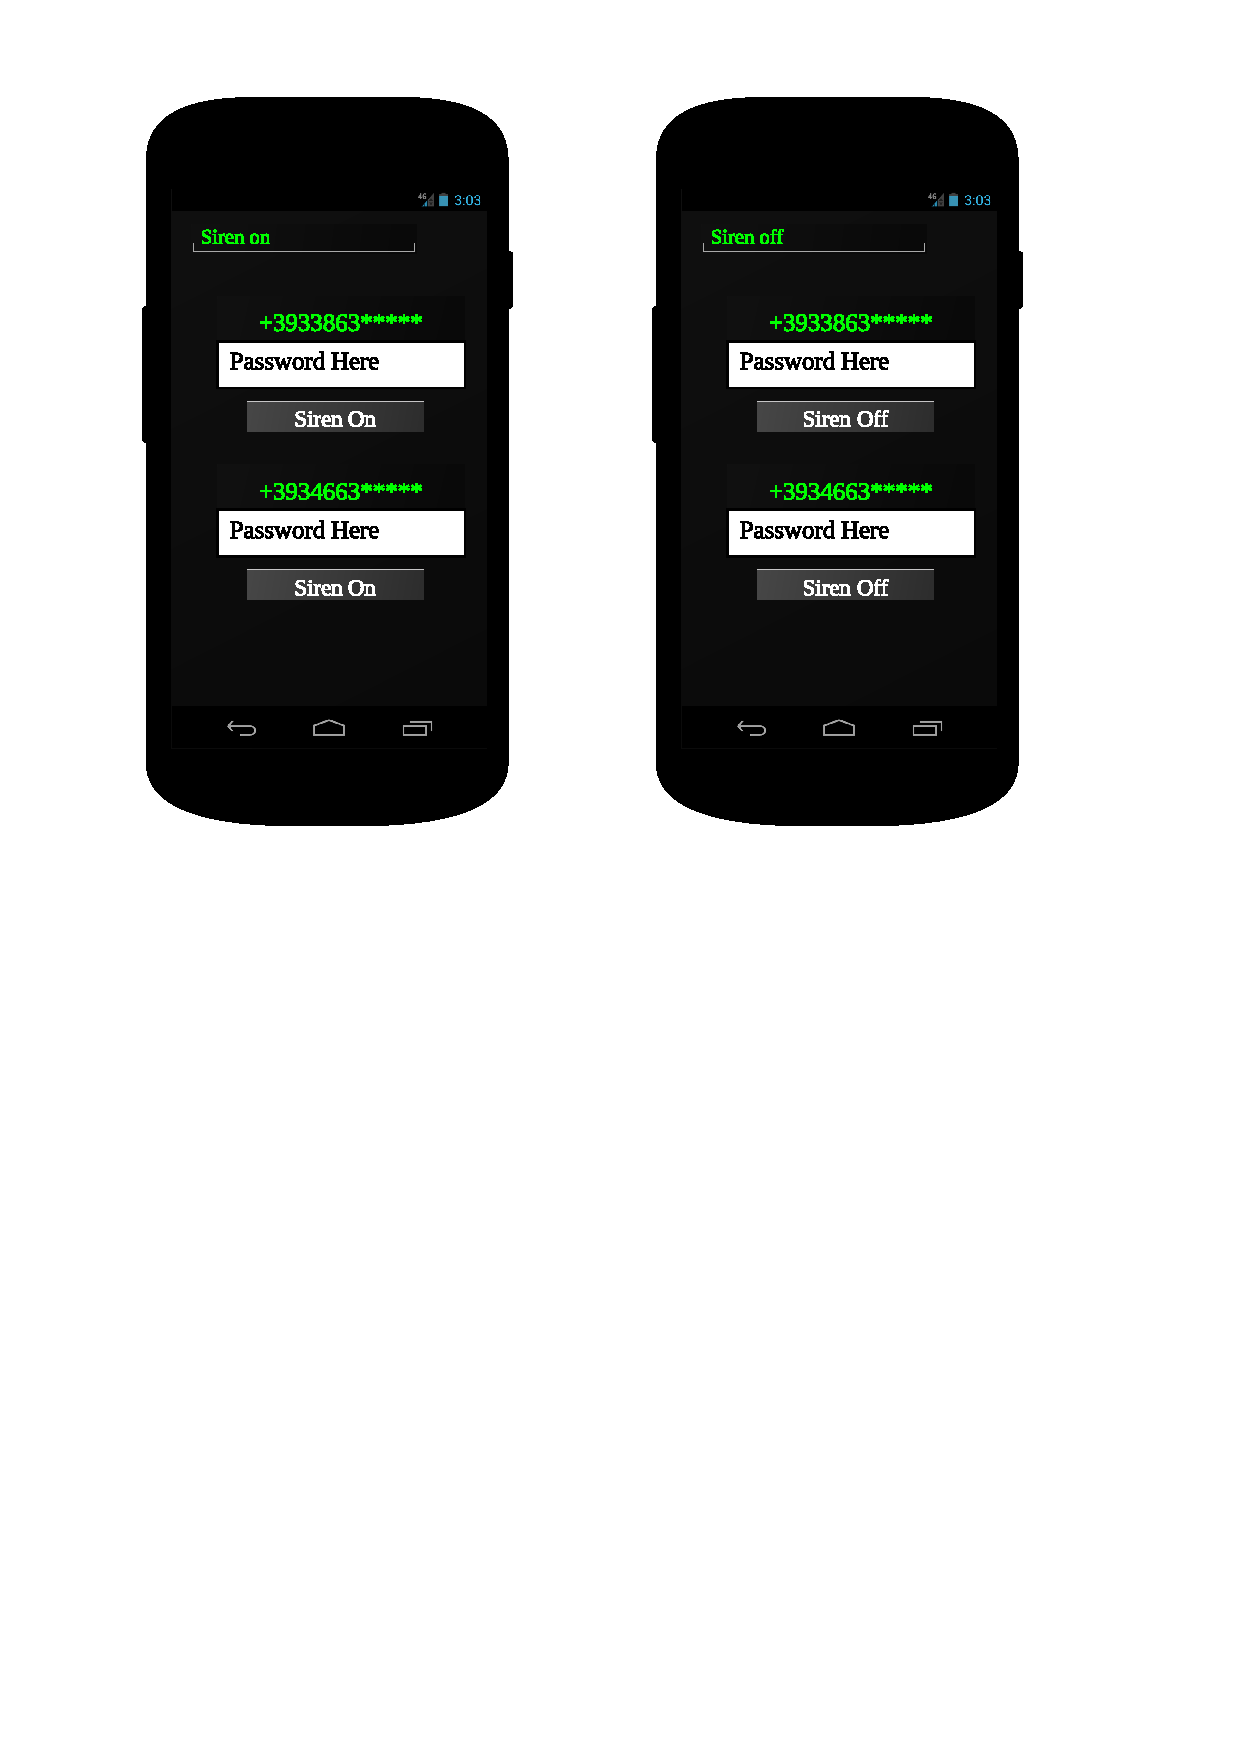
\includegraphics[scale=0.7]{images/sirenonoff_mobile}


\section{Perimeter Selection}

The perimeter selection feature, when activated, must select a circle area
centered where the cellphone is at that moment, and trigger an alarm if the
mobile phone exits from there. The circular limit has also to be visible on a
map on the telephone.


\newpage
\subsection{Activity Diagram}

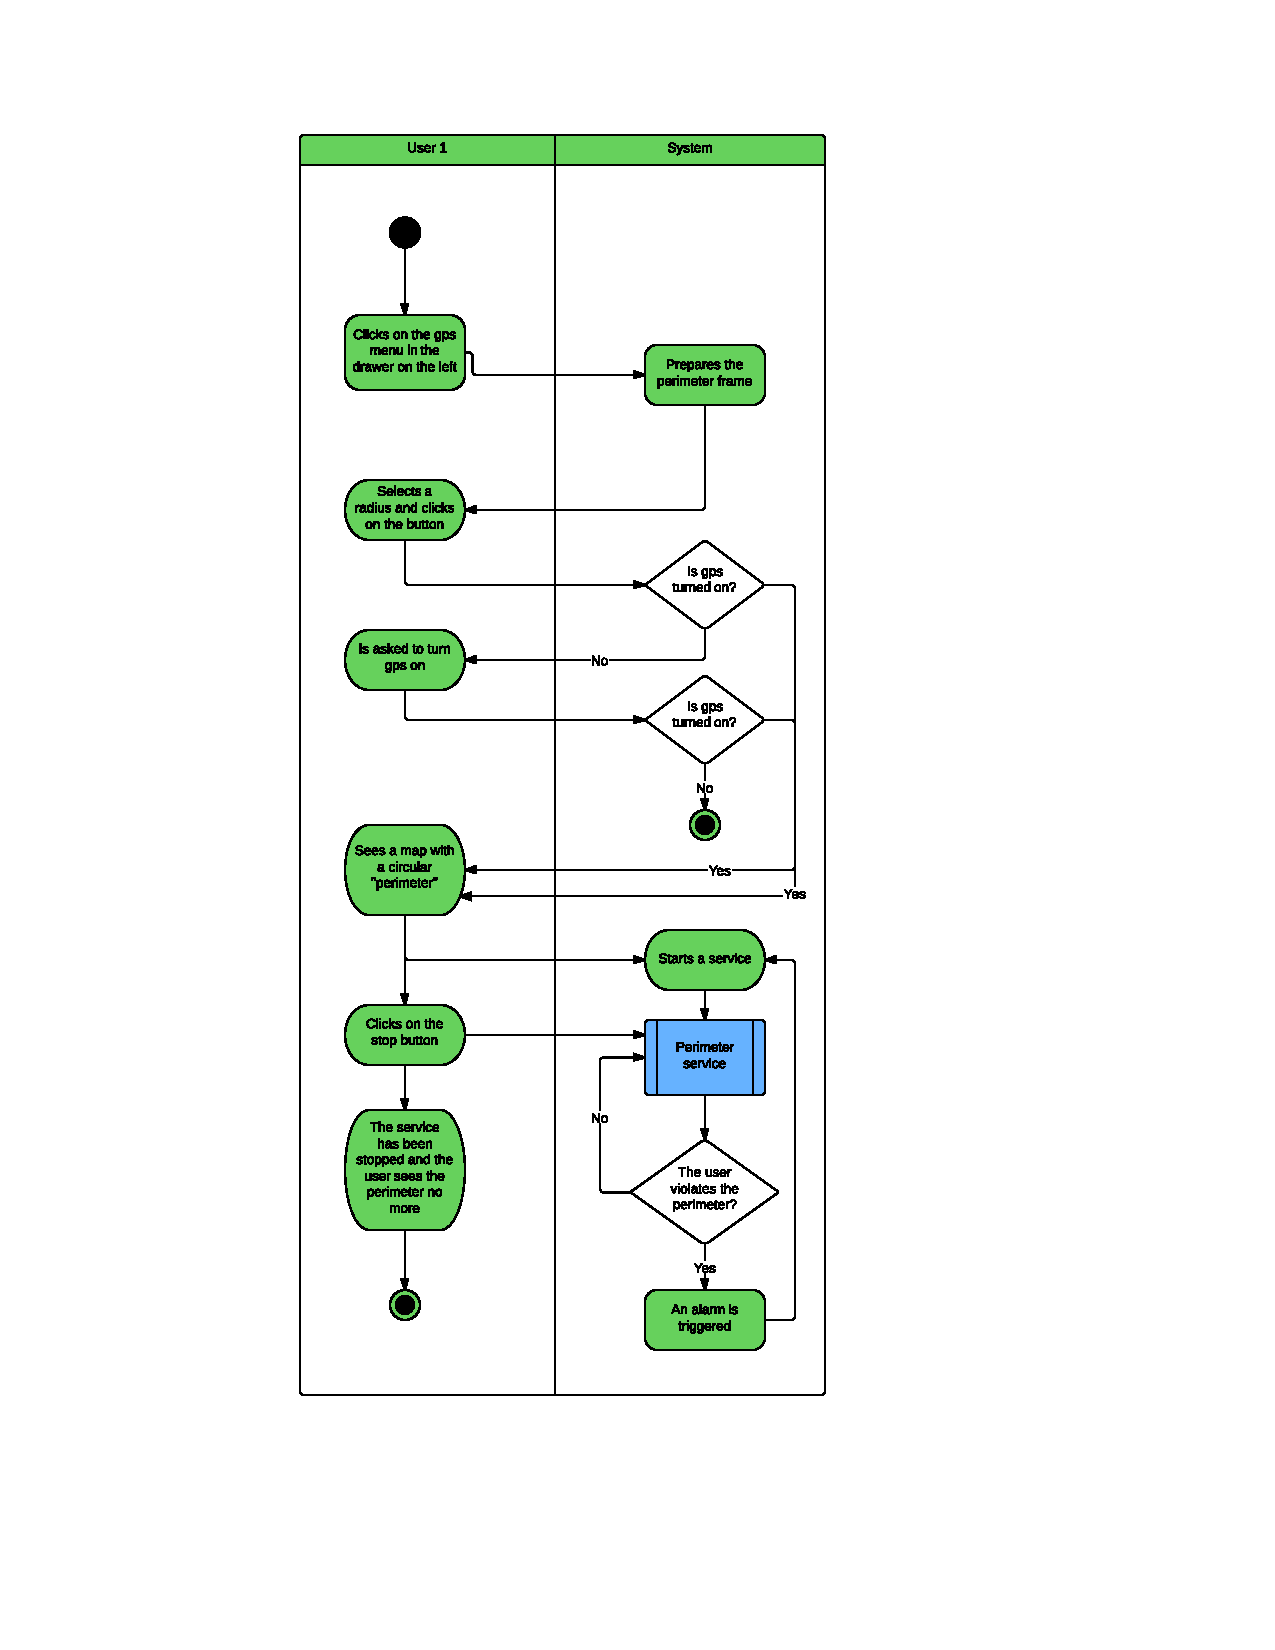
\includegraphics[scale=0.7]{images/Perimeter}

\newpage
\subsection{User Interface Design}

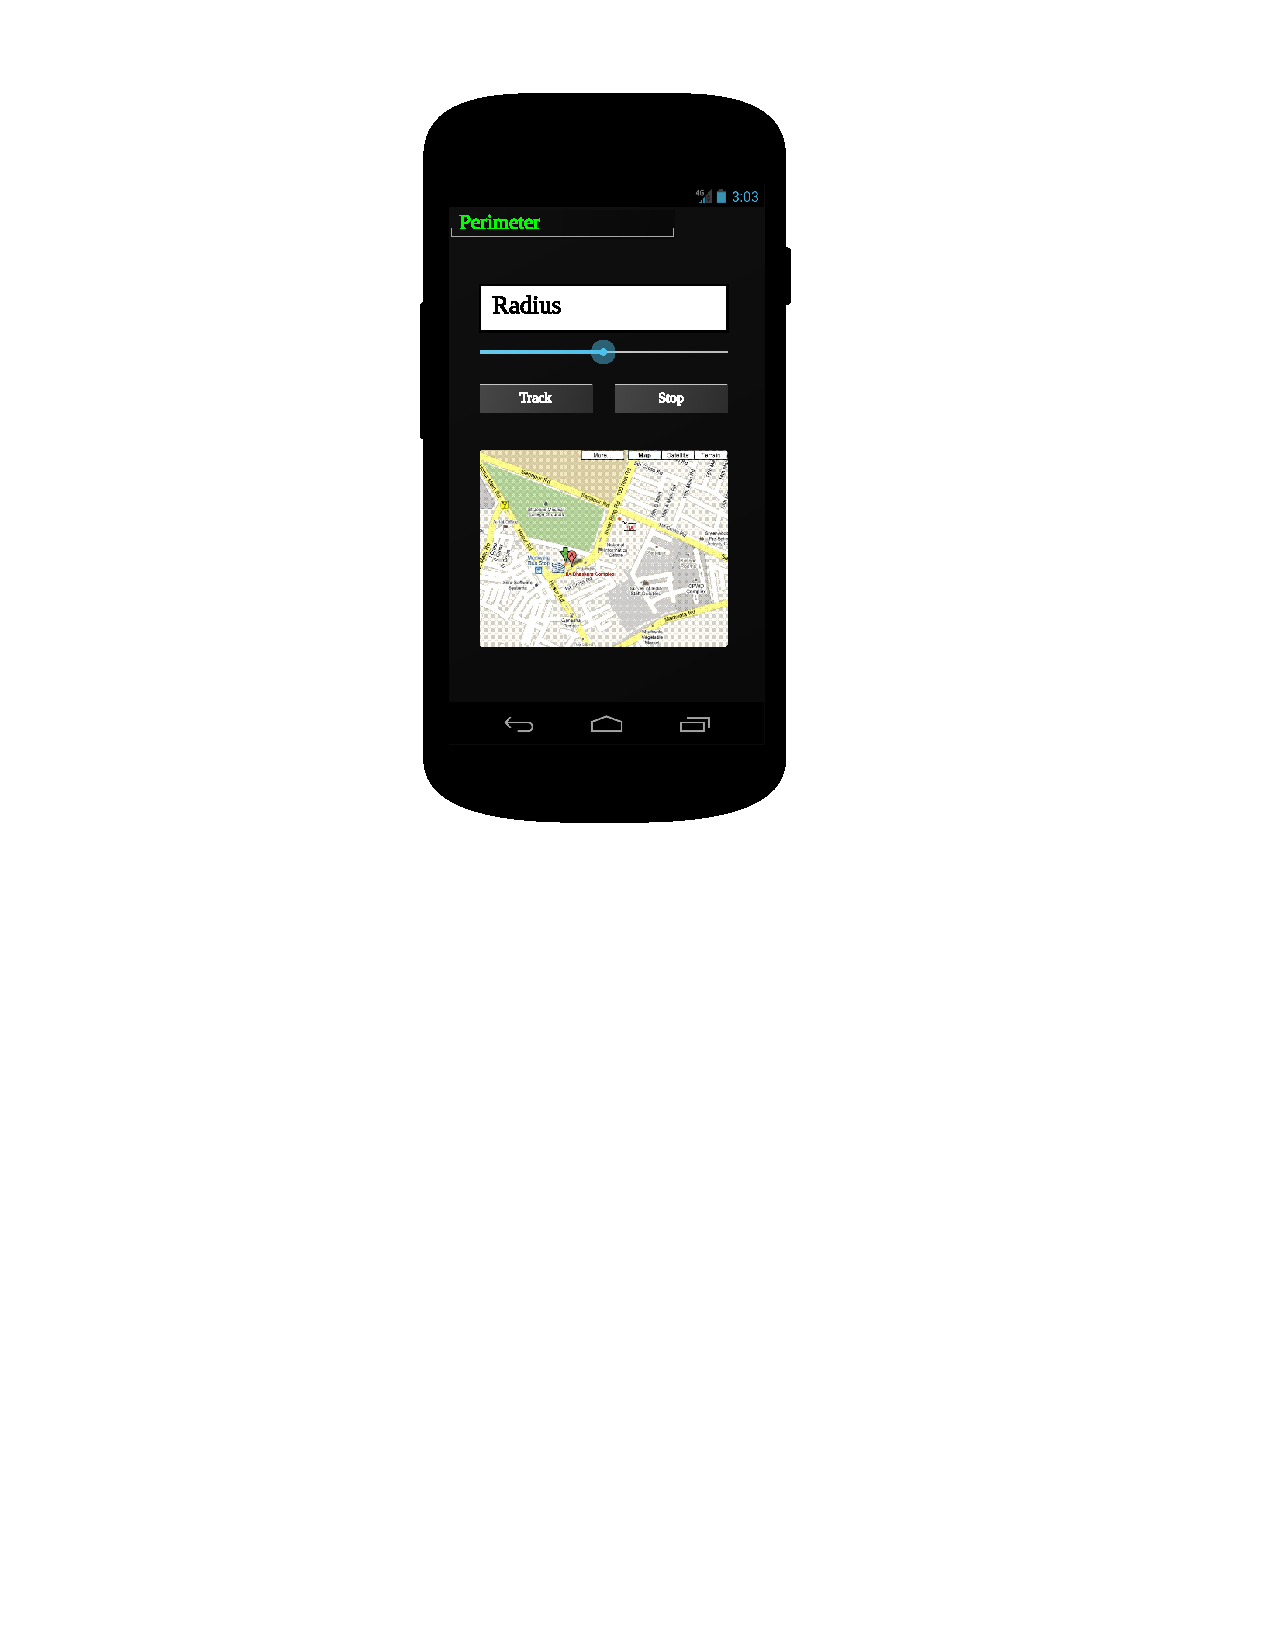
\includegraphics[scale=0.7]{images/Perimeter_mobile}
